\section{Analyse}

\subsection{Fonctionnement général}

Au lancement du jeu, le joueur peut choisir de lancer un partie ou de quitter le jeu. Lors de versions ultérieurs, d'autres options pourraient s'ajouter dans ce menu, comme des options ou des parties en ligne.

\begin{figure}[h]
  \centering
  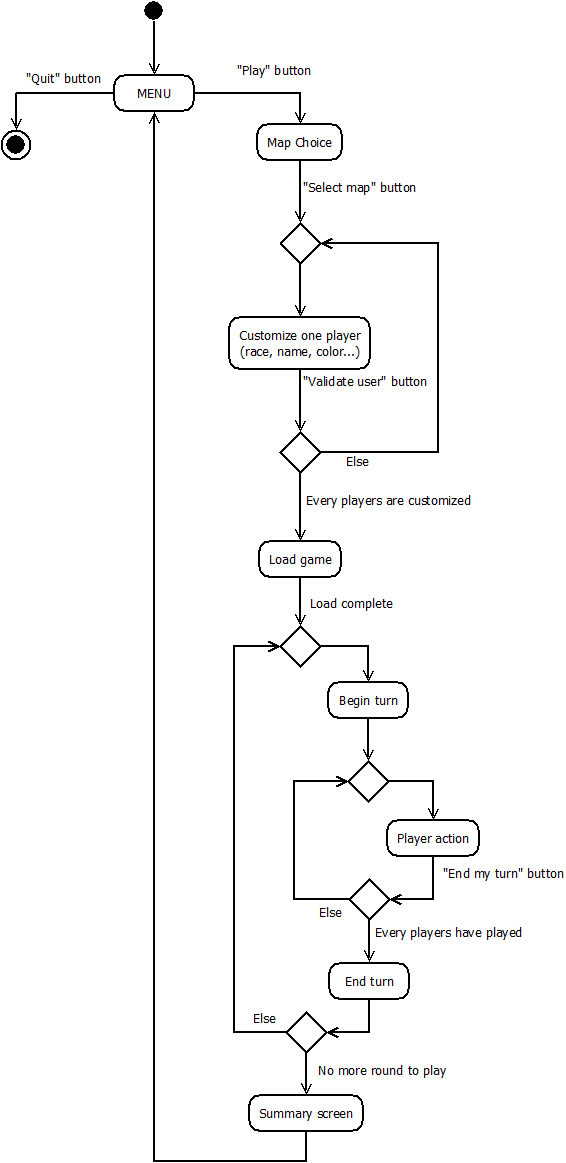
\includegraphics[width=5cm]{schemas/activity.png}
  \caption{Diagramme d'activité}
  \label{activity}
\end{figure}




\subsection{Créer ou charger une partie}

Lorsque le joueur veut lancer un partie, il peut au choix

\begin{figure}[h]
  \centering
  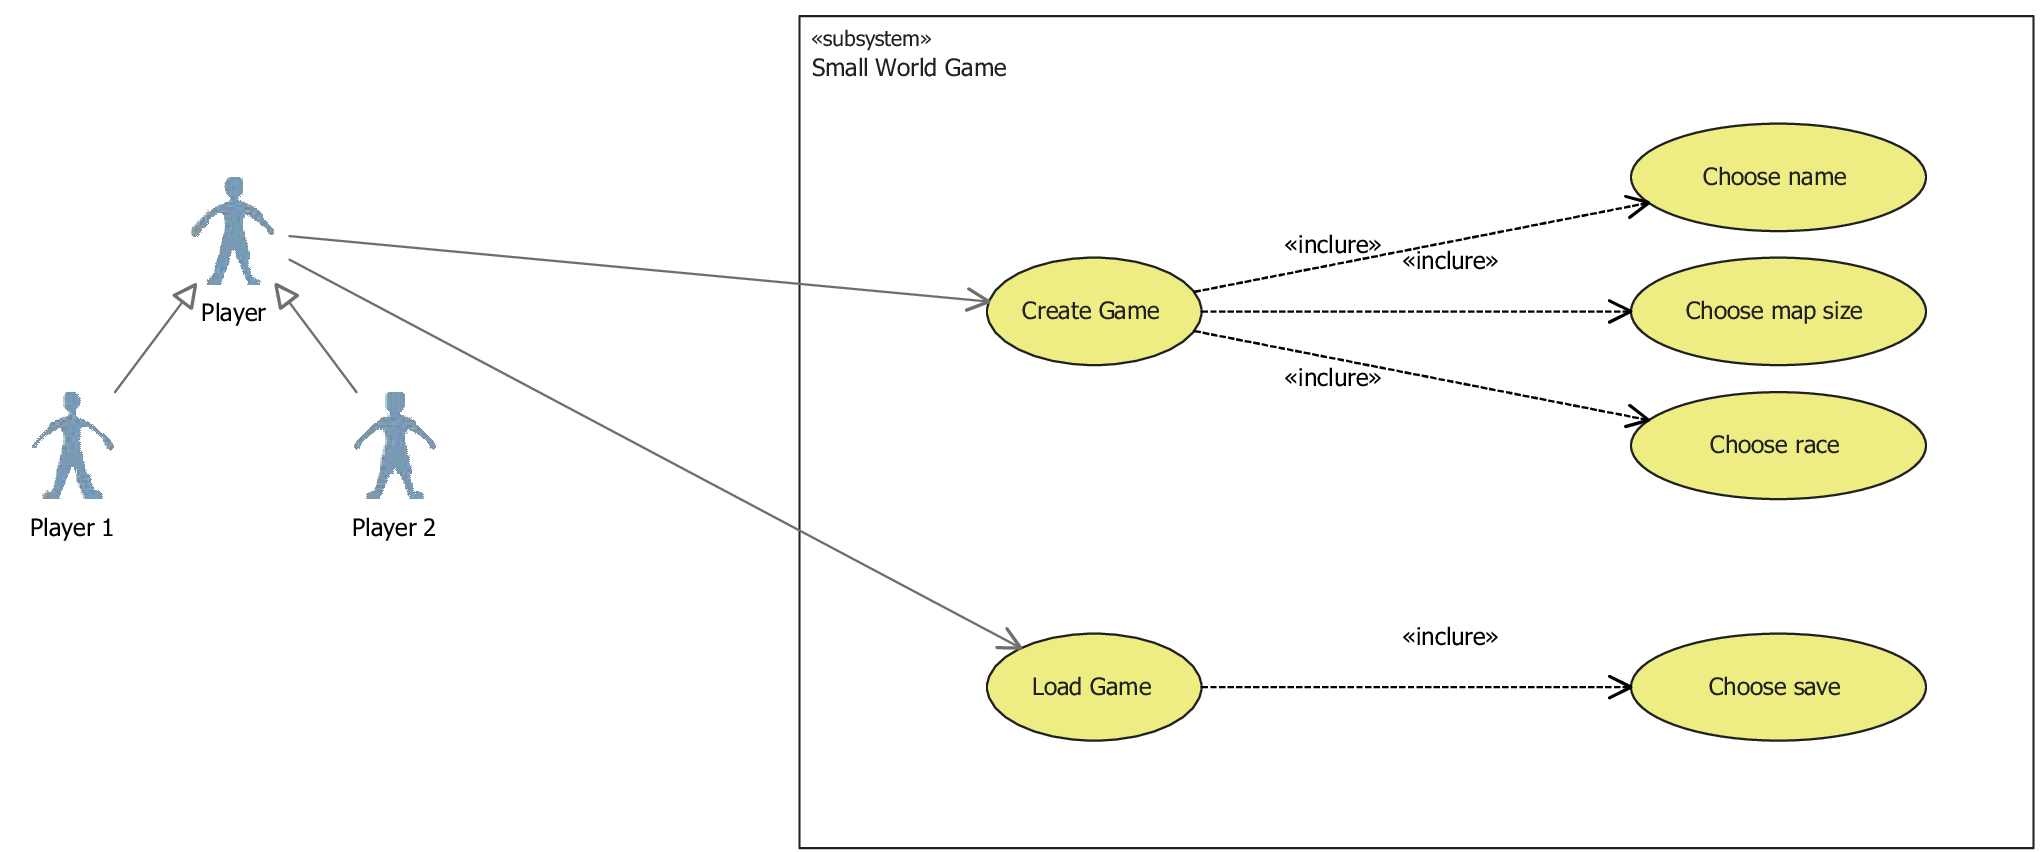
\includegraphics[width=13cm]{schemas/uc_game_creation.png}
  \caption{Diagramme de cas d'utilisation du lancement d'une partie}
  \label{uc_game_creation}
\end{figure}


\subsection{Déroulement d'un tour de jeu}
\subsubsection{Gestion des déplacements}
\subsubsection{Gestion des combats}

\subsection{Cycle de vie d'une unité}

\begin{figure}[!h]
  \centering
  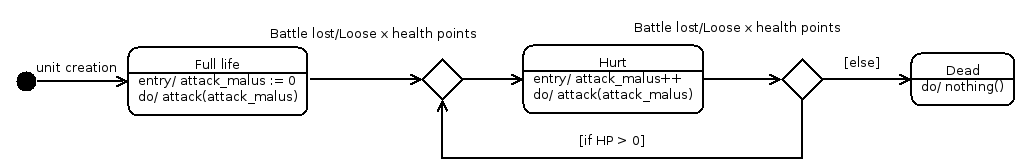
\includegraphics[width=13cm]{schemas/state-diagram.png}
  \caption{Cycle de vie d'une unité}
  \label{state-diagram}
\end{figure}


